\section{Initial Optimization}
This section describes the initial optimization on the simplified problem with two variables. All other variables were set to constant values in the feasible domain. 
\subsection{Straight Design}
Two variables: $w_b$ and $F$ were optimized to investigate the implementation of the SQP algorithm. The other variables, $h_f$, $v_a$ and $v_b$ were set to 1.0, 2.0 and 1.0 respectively such that these lie inside the feasible domain. The starting point was set to $[w_b F] = [1, 1]$ and the SQP algorithm was executed. The result is shown in \autoref{fig:straightopt}. As can be seen, the algorithm converges along constraint $g_{ca}$ towards the optimum of $[w_b F] = [2.25 23.56]$ mm, N. The minimized value of the objective function is then 0.145 mm$^2$/N, thus the maximum strength equals 6.90 N/mm$^2$ for this configuration. Constraints $g_{ca}$ and $g_{tb}$ are active. It takes 152 iterations till convergence. The SQP algorithm iterates in the infeasible domain as well, however this was as expected.


\begin{figure}[H]
	\centering
	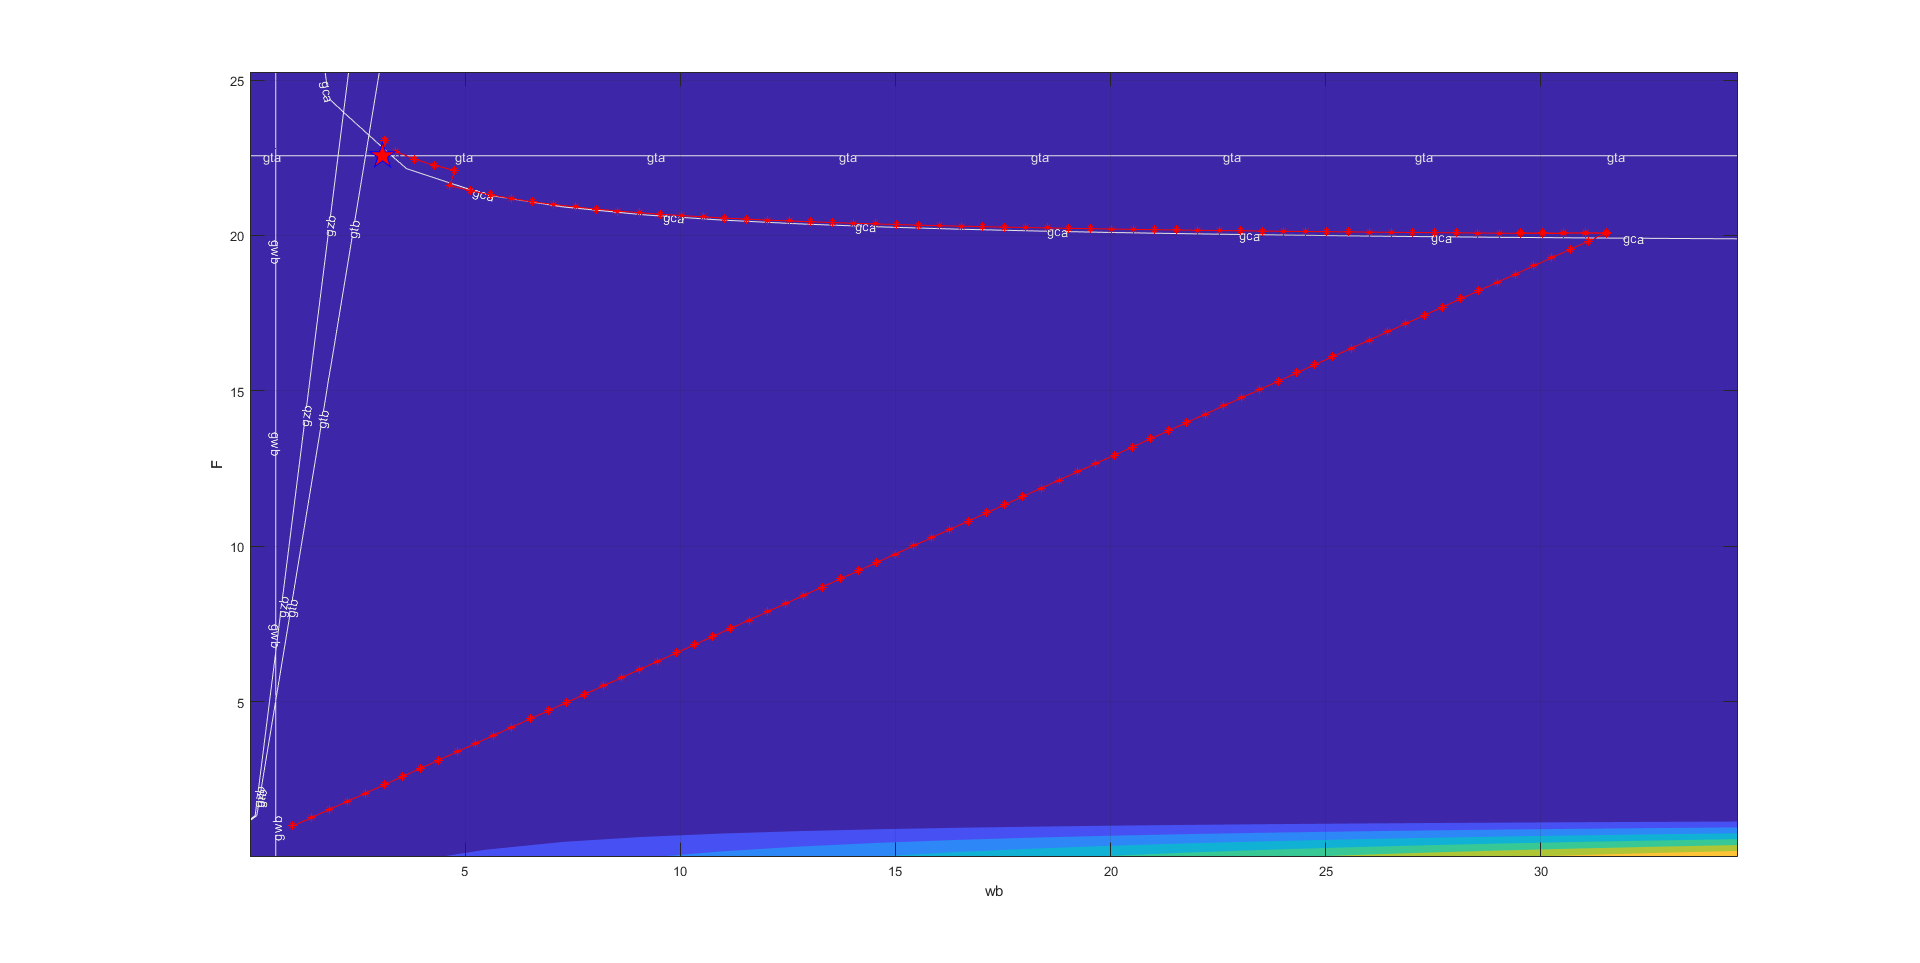
\includegraphics[width=\columnwidth]{sources/plots/straight2var.png}
	\caption{The optimization steps taken by the SQP algorithm for the design variables $w_b$ and $F$ in the straight design. The dashed line shows the infeasible domain.}
	\label{fig:straightopt}
\end{figure}


The KKT conditions were also checked. The feasibility conditions are satisfied because all inequality constraints are smaller than zero. Constraints $g_{ca}$ and $g_{tb}$ are treated as active, setting $\frac{\partial L}{\partial x} = 0$ gives two Lagrangian multipliers $\mu$ of 0.03 and 0.116. Since $\mu$ > 0, the KKT conditions are satisfied. Still, since not all constraint functions are convex, we cannot conclude that this is the global optimum from the KKT conditions merely. However, when looking at contour plot, the found optimum seems to be the global optimum since it lies just in the feasible domain and minimizes the objective function. 


\subsection{Diagonal Design}
The same SQP algorithm was also tested on the diagonal design. Again, $w_b$ and $F$ were optimized with an initial value of $[w_b F] = [1, 1]$. The other design variables $w_a$ and $L$ were set to 1.0 and 3.0 respectively. \autoref{fig:diagopt} shows the result, where $w_b$ and $F$ converge to 2.36 mm and 4.59 N respectively. This gives a minimized objective of 0.732 mm$^2$/N, equal to a maximum strength of 1.37 N/mm$^2$. Constraint $g_{5a}$ and $g_{5b}$ are then active and it takes 21 iterations till the optimum is found.


\begin{figure}[H]
	\centering
	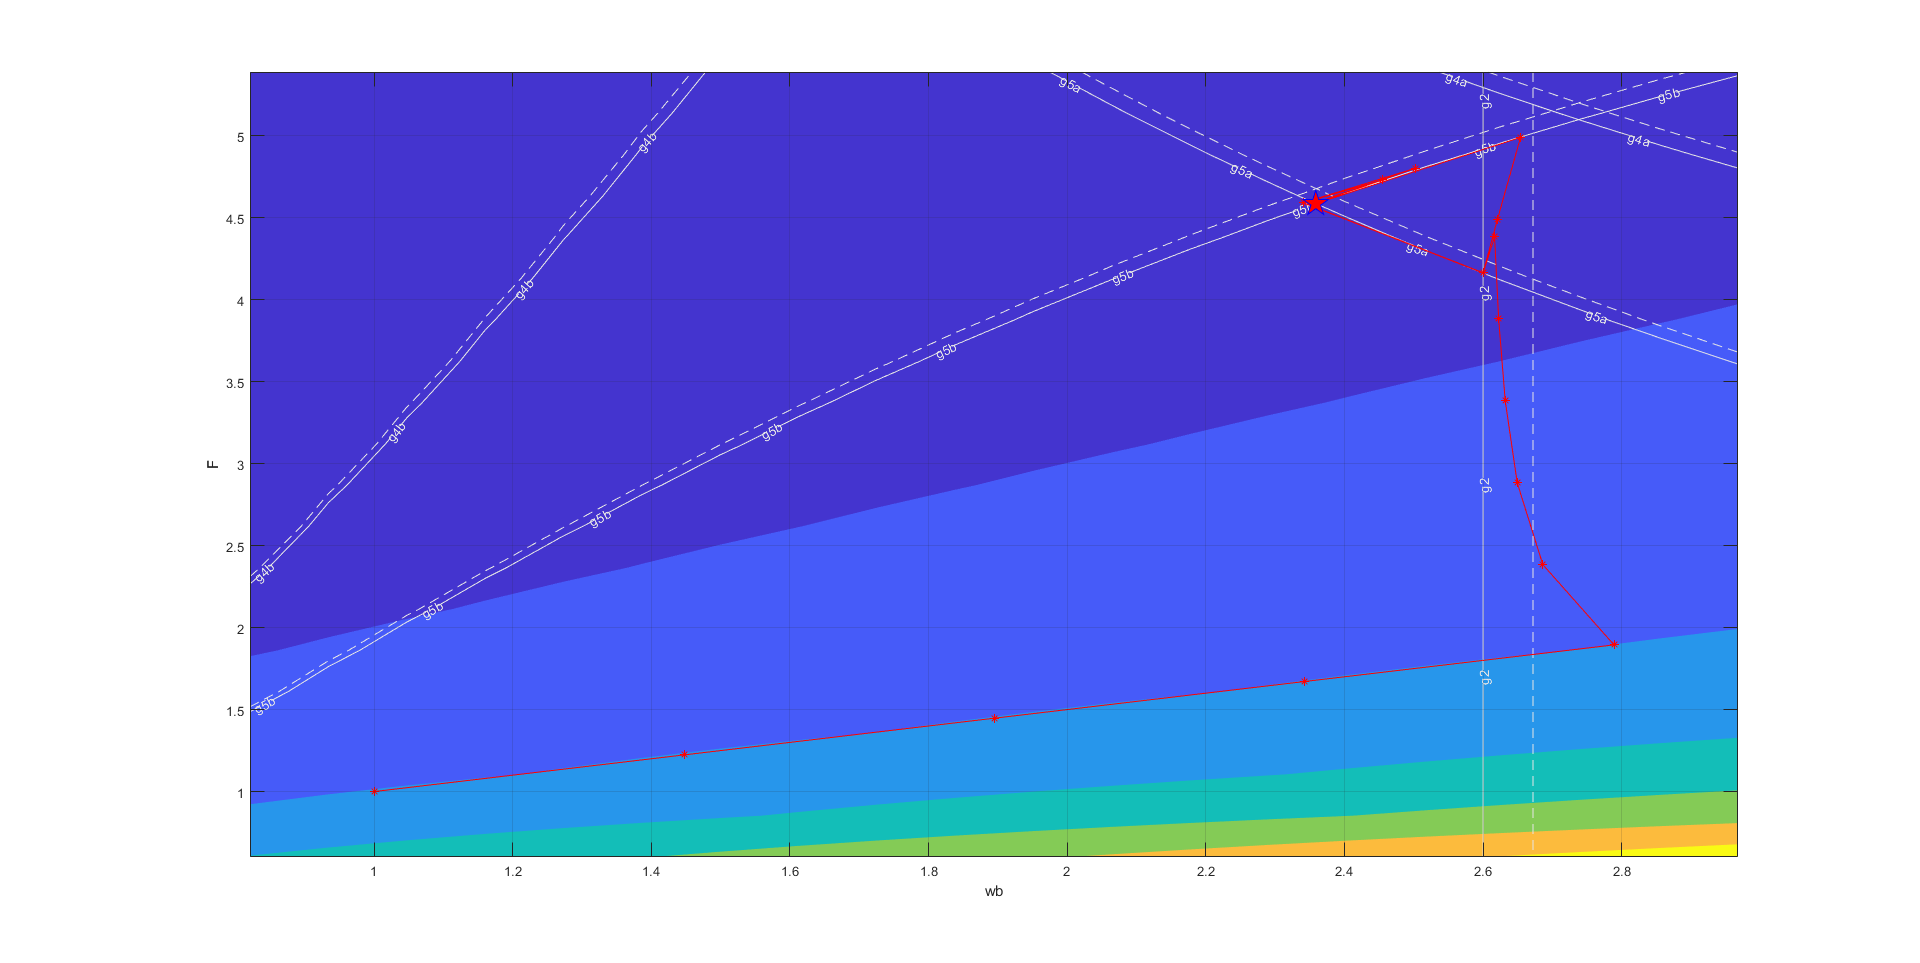
\includegraphics[width=\columnwidth]{sources/plots/diagonal2var.png}
	\caption{The optimization steps taken by the SQP algorithm for the design variables $w_b$ and $F$ in the diagonal design. The dashed line shows the infeasible domain.}
	\label{fig:diagopt}
\end{figure}

Looking at the KKT conditions, the optimum lies in the feasible domain since all inequality constraints are smaller than zero, and therefore satisfied. Treating constraints $g_{5a}$ and $g_{5b}$ as active gives two Lagrangian multipliers $\mu$ of 0.15 and 0.73. Since $\mu$ > 0, the KKT conditions are satisfied and the SQP algorithm has found a local optimum. Still, the constraints are not convex so it cannot be concluded that this is a global optimum from the KKT conditions only. Observing the contour plot, it can be seen that the objective function is minimized at the optimum found, and all constraints are satisfied. Therefore, the SQP algorithm found a global optimum in this case as well.\\

Note that the maximum strength values for the straight vs diagonal design are not comparable yet, since the other design variables were set at an arbitrary value in the feasible domain.








